% Options for packages loaded elsewhere
\PassOptionsToPackage{unicode}{hyperref}
\PassOptionsToPackage{hyphens}{url}
%
\documentclass[
  french,
]{article}
\usepackage{amsmath,amssymb}
\usepackage{lmodern}
\usepackage{ifxetex,ifluatex}
\ifnum 0\ifxetex 1\fi\ifluatex 1\fi=0 % if pdftex
  \usepackage[T1]{fontenc}
  \usepackage[utf8]{inputenc}
  \usepackage{textcomp} % provide euro and other symbols
\else % if luatex or xetex
  \usepackage{unicode-math}
  \defaultfontfeatures{Scale=MatchLowercase}
  \defaultfontfeatures[\rmfamily]{Ligatures=TeX,Scale=1}
\fi
% Use upquote if available, for straight quotes in verbatim environments
\IfFileExists{upquote.sty}{\usepackage{upquote}}{}
\IfFileExists{microtype.sty}{% use microtype if available
  \usepackage[]{microtype}
  \UseMicrotypeSet[protrusion]{basicmath} % disable protrusion for tt fonts
}{}
\makeatletter
\@ifundefined{KOMAClassName}{% if non-KOMA class
  \IfFileExists{parskip.sty}{%
    \usepackage{parskip}
  }{% else
    \setlength{\parindent}{0pt}
    \setlength{\parskip}{6pt plus 2pt minus 1pt}}
}{% if KOMA class
  \KOMAoptions{parskip=half}}
\makeatother
\usepackage{xcolor}
\IfFileExists{xurl.sty}{\usepackage{xurl}}{} % add URL line breaks if available
\IfFileExists{bookmark.sty}{\usepackage{bookmark}}{\usepackage{hyperref}}
\hypersetup{
  pdftitle={Essai d'article complet avec toutes les contraintes},
  pdfauthor={Nicolas Bressoud},
  pdflang={fr},
  hidelinks,
  pdfcreator={LaTeX via pandoc}}
\urlstyle{same} % disable monospaced font for URLs
\usepackage[margin=1in]{geometry}
\usepackage{color}
\usepackage{fancyvrb}
\newcommand{\VerbBar}{|}
\newcommand{\VERB}{\Verb[commandchars=\\\{\}]}
\DefineVerbatimEnvironment{Highlighting}{Verbatim}{commandchars=\\\{\}}
% Add ',fontsize=\small' for more characters per line
\usepackage{framed}
\definecolor{shadecolor}{RGB}{248,248,248}
\newenvironment{Shaded}{\begin{snugshade}}{\end{snugshade}}
\newcommand{\AlertTok}[1]{\textcolor[rgb]{0.94,0.16,0.16}{#1}}
\newcommand{\AnnotationTok}[1]{\textcolor[rgb]{0.56,0.35,0.01}{\textbf{\textit{#1}}}}
\newcommand{\AttributeTok}[1]{\textcolor[rgb]{0.77,0.63,0.00}{#1}}
\newcommand{\BaseNTok}[1]{\textcolor[rgb]{0.00,0.00,0.81}{#1}}
\newcommand{\BuiltInTok}[1]{#1}
\newcommand{\CharTok}[1]{\textcolor[rgb]{0.31,0.60,0.02}{#1}}
\newcommand{\CommentTok}[1]{\textcolor[rgb]{0.56,0.35,0.01}{\textit{#1}}}
\newcommand{\CommentVarTok}[1]{\textcolor[rgb]{0.56,0.35,0.01}{\textbf{\textit{#1}}}}
\newcommand{\ConstantTok}[1]{\textcolor[rgb]{0.00,0.00,0.00}{#1}}
\newcommand{\ControlFlowTok}[1]{\textcolor[rgb]{0.13,0.29,0.53}{\textbf{#1}}}
\newcommand{\DataTypeTok}[1]{\textcolor[rgb]{0.13,0.29,0.53}{#1}}
\newcommand{\DecValTok}[1]{\textcolor[rgb]{0.00,0.00,0.81}{#1}}
\newcommand{\DocumentationTok}[1]{\textcolor[rgb]{0.56,0.35,0.01}{\textbf{\textit{#1}}}}
\newcommand{\ErrorTok}[1]{\textcolor[rgb]{0.64,0.00,0.00}{\textbf{#1}}}
\newcommand{\ExtensionTok}[1]{#1}
\newcommand{\FloatTok}[1]{\textcolor[rgb]{0.00,0.00,0.81}{#1}}
\newcommand{\FunctionTok}[1]{\textcolor[rgb]{0.00,0.00,0.00}{#1}}
\newcommand{\ImportTok}[1]{#1}
\newcommand{\InformationTok}[1]{\textcolor[rgb]{0.56,0.35,0.01}{\textbf{\textit{#1}}}}
\newcommand{\KeywordTok}[1]{\textcolor[rgb]{0.13,0.29,0.53}{\textbf{#1}}}
\newcommand{\NormalTok}[1]{#1}
\newcommand{\OperatorTok}[1]{\textcolor[rgb]{0.81,0.36,0.00}{\textbf{#1}}}
\newcommand{\OtherTok}[1]{\textcolor[rgb]{0.56,0.35,0.01}{#1}}
\newcommand{\PreprocessorTok}[1]{\textcolor[rgb]{0.56,0.35,0.01}{\textit{#1}}}
\newcommand{\RegionMarkerTok}[1]{#1}
\newcommand{\SpecialCharTok}[1]{\textcolor[rgb]{0.00,0.00,0.00}{#1}}
\newcommand{\SpecialStringTok}[1]{\textcolor[rgb]{0.31,0.60,0.02}{#1}}
\newcommand{\StringTok}[1]{\textcolor[rgb]{0.31,0.60,0.02}{#1}}
\newcommand{\VariableTok}[1]{\textcolor[rgb]{0.00,0.00,0.00}{#1}}
\newcommand{\VerbatimStringTok}[1]{\textcolor[rgb]{0.31,0.60,0.02}{#1}}
\newcommand{\WarningTok}[1]{\textcolor[rgb]{0.56,0.35,0.01}{\textbf{\textit{#1}}}}
\usepackage{longtable,booktabs,array}
\usepackage{calc} % for calculating minipage widths
% Correct order of tables after \paragraph or \subparagraph
\usepackage{etoolbox}
\makeatletter
\patchcmd\longtable{\par}{\if@noskipsec\mbox{}\fi\par}{}{}
\makeatother
% Allow footnotes in longtable head/foot
\IfFileExists{footnotehyper.sty}{\usepackage{footnotehyper}}{\usepackage{footnote}}
\makesavenoteenv{longtable}
\usepackage{graphicx}
\makeatletter
\def\maxwidth{\ifdim\Gin@nat@width>\linewidth\linewidth\else\Gin@nat@width\fi}
\def\maxheight{\ifdim\Gin@nat@height>\textheight\textheight\else\Gin@nat@height\fi}
\makeatother
% Scale images if necessary, so that they will not overflow the page
% margins by default, and it is still possible to overwrite the defaults
% using explicit options in \includegraphics[width, height, ...]{}
\setkeys{Gin}{width=\maxwidth,height=\maxheight,keepaspectratio}
% Set default figure placement to htbp
\makeatletter
\def\fps@figure{htbp}
\makeatother
\setlength{\emergencystretch}{3em} % prevent overfull lines
\providecommand{\tightlist}{%
  \setlength{\itemsep}{0pt}\setlength{\parskip}{0pt}}
\setcounter{secnumdepth}{5}
\ifxetex
  % Load polyglossia as late as possible: uses bidi with RTL langages (e.g. Hebrew, Arabic)
  \usepackage{polyglossia}
  \setmainlanguage[]{french}
\else
  \usepackage[main=french]{babel}
% get rid of language-specific shorthands (see #6817):
\let\LanguageShortHands\languageshorthands
\def\languageshorthands#1{}
\fi
\ifluatex
  \usepackage{selnolig}  % disable illegal ligatures
\fi
\newlength{\cslhangindent}
\setlength{\cslhangindent}{1.5em}
\newlength{\csllabelwidth}
\setlength{\csllabelwidth}{3em}
\newenvironment{CSLReferences}[2] % #1 hanging-ident, #2 entry spacing
 {% don't indent paragraphs
  \setlength{\parindent}{0pt}
  % turn on hanging indent if param 1 is 1
  \ifodd #1 \everypar{\setlength{\hangindent}{\cslhangindent}}\ignorespaces\fi
  % set entry spacing
  \ifnum #2 > 0
  \setlength{\parskip}{#2\baselineskip}
  \fi
 }%
 {}
\usepackage{calc}
\newcommand{\CSLBlock}[1]{#1\hfill\break}
\newcommand{\CSLLeftMargin}[1]{\parbox[t]{\csllabelwidth}{#1}}
\newcommand{\CSLRightInline}[1]{\parbox[t]{\linewidth - \csllabelwidth}{#1}\break}
\newcommand{\CSLIndent}[1]{\hspace{\cslhangindent}#1}

\title{Essai d'article complet avec toutes les contraintes}
\author{Nicolas Bressoud}
\date{juin 2020}

\begin{document}
\maketitle

\renewcommand*\contentsname{Table des matières}
{
\setcounter{tocdepth}{2}
\tableofcontents
}
\hypertarget{titre-de-niveau-1-salut}{%
\section{Titre de niveau 1 salut}\label{titre-de-niveau-1-salut}}

\begin{itemize}
\tightlist
\item
  ajouter image interne (générée par R) avec référence dans le texte, légende
\item
  ajouter table avec référence dans le texte, légende (kable)
\item
  ajouter image externe, avec référence dans le texte, légende
\item
  ajouter référence biblio dans texte
\item
  ajouter biblio
\end{itemize}

PDF et Word énumèrent pas.

\begin{quote}
à gérer la langue de ``table of contents'' et ``table'' au lieu de ``tableau''.
\end{quote}

\hypertarget{tableau}{%
\section{tableau}\label{tableau}}

Si on se réfère au tableau \ref{tab:iris-lol}, on voit que c'est beau. Ou \ref{tab:table-single}

\begin{table}

\caption{\label{tab:iris-lol}A table of the first 10 rows of the mtcars data.}
\centering
\begin{tabular}[t]{r|r|r|r|l}
\hline
Sepal Length & Sepal Width & Petal Length & Petal Width & Species\\
\hline
5.1 & 3.5 & 1.4 & 0.2 & setosa\\
\hline
4.9 & 3.0 & 1.4 & 0.2 & setosa\\
\hline
4.7 & 3.2 & 1.3 & 0.2 & setosa\\
\hline
4.6 & 3.1 & 1.5 & 0.2 & setosa\\
\hline
5.0 & 3.6 & 1.4 & 0.2 & setosa\\
\hline
5.4 & 3.9 & 1.7 & 0.4 & setosa\\
\hline
\end{tabular}
\end{table}

\begin{table}

\caption{\label{tab:table-single}A table of the first 10 rows of the mtcars data.}
\centering
\begin{tabular}[t]{rrrrl}
\toprule
Sepal.Length & Sepal.Width & Petal.Length & Petal.Width & Species\\
\midrule
5.1 & 3.5 & 1.4 & 0.2 & setosa\\
4.9 & 3.0 & 1.4 & 0.2 & setosa\\
4.7 & 3.2 & 1.3 & 0.2 & setosa\\
4.6 & 3.1 & 1.5 & 0.2 & setosa\\
5.0 & 3.6 & 1.4 & 0.2 & setosa\\
\addlinespace
5.4 & 3.9 & 1.7 & 0.4 & setosa\\
\bottomrule
\end{tabular}
\end{table}

La mise en forme et l'emplacement des tableaux diffèrent selon le type de sorties. Voir aussi Andy Field pour ajouter du KableExtra ?

WORD fait pas de différences entre les deux mises en page de tableaux.

\hypertarget{image-interne}{%
\section{image interne}\label{image-interne}}

Si on se réfère à l'image interne \ref{fig:pressure}, on voit que c'est beau.

\begin{Shaded}
\begin{Highlighting}[]
\FunctionTok{plot}\NormalTok{(pressure)}
\end{Highlighting}
\end{Shaded}

\begin{figure}
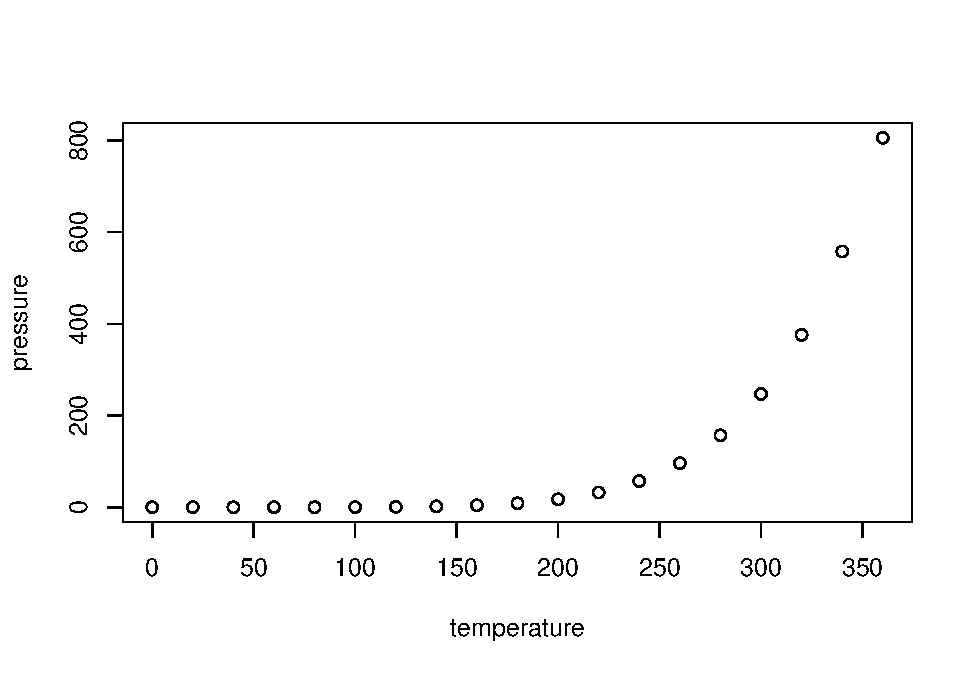
\includegraphics[width=0.7\linewidth]{essai_files/figure-latex/pressure-1} \caption{A figure example with a relative width 70\%.}\label{fig:pressure}
\end{figure}

\hypertarget{image-externe}{%
\section{Image externe}\label{image-externe}}

Figure \ref{fig:knitr-logo} is an example of three \textbf{knitr} logos included in a figure environment.

\begin{figure}

\includegraphics[width=0.328\linewidth]{images/knit-logo} 
\includegraphics[width=0.328\linewidth]{images/knit-logo} 
\includegraphics[width=0.328\linewidth]{images/knit-logo} \caption{Three knitr logos included in the document from an external PNG image file.}\label{fig:knitr-logo}
\end{figure}

Word réduit pas les tailles.

\hypertarget{citations}{%
\section{Citations}\label{citations}}

La vie est belle (Rébecca Shankland, 2015 ; R. Shankland \& Lamboy, 2011). Et aime bien le discours de Shankland (2015). Rébecca Shankland (2012) pense aussi cela. Mais pas tout le temps (voir Rébecca Shankland, 2015, pp.~33-35, également 2012, ch.~1). Salut la vie (Rebecca Shankland et al., 2018).

\hypertarget{biblio}{%
\section{Biblio}\label{biblio}}

Biblio doit contenir les 4 références :
Mais aussi voir pour faire la biblio d'office en entier à partir du fichier bibtex (bio CV).

\hypertarget{refs}{}
\begin{CSLReferences}{1}{0}
\leavevmode\hypertarget{ref-shankland2012}{}%
Shankland, Rébecca. (2012). Bien-Être Subjectif et Comportements Altruistes : Les Individus Heureux Sont-Ils plus Généreux ? \emph{Cips}, \emph{n{}}, 77‑88. \url{https://doi.org/10.3917/cips.093.0077}

\leavevmode\hypertarget{ref-shankland2015}{}%
Shankland, Rébecca. (2015). \emph{La Psychologie Positive}. {Dunod}.

\leavevmode\hypertarget{ref-shankland2018a}{}%
Shankland, Rebecca, Bressoud, N., Tessier, D., \& Gay, P. (2018). La Bienveillance~: Une Compétence Socio-Émotionnelle de l'enseignant Au Service Du Bien-Être et Des Apprentissages~? \emph{Questions vives recherches en éducation}, \emph{N{} 29}, 0‑23. \url{https://doi.org/10.4000/questionsvives.3601}

\leavevmode\hypertarget{ref-shankland2011}{}%
Shankland, R., \& Lamboy, B. (2011). Utilité Des Modles Théoriques Pour La Conception et l'évaluation de Programmes En Prévention et Promotion de La Santé. \emph{Pratiques Psychologiques}, \emph{17}(2), 153‑172. \url{https://doi.org/10.1016/j.prps.2010.11.001}

\end{CSLReferences}

\end{document}
